\chapter{Detector Combination} \label{chapter2}




 \section{Boolean Combination of Detectors in the ROC Space}
\label{sec:boolean-combination}

This section provides information about ROC analysis and summarizes the Boolean combination in the ROC space \cite{Khreich2010-ICPR}.
A crisp detector outputs a decision or a class label (e.g., normal or anomaly) while a soft detector such as HMM assigns scores to the input samples, which can be converted to a crisp detector by setting a decision threshold on the scores.
Given the responses of a crisp detector on a validation set, the true positive rate ($tpr$) is the proportion of positives correctly classified over the total number of positive samples.
The false positive rate ($fpr$) is the proportion of negatives incorrectly classified over the total number of negative samples.
The positive (or target) class is typically the class of interest, which is the anomalous class for an ADS.

A ROC curve is a plot of $tpr$ against $fpr$ \cite{Fawcett2006}.
A crisp detector produces a single data point in the ROC space, while a soft detector produces a ROC curve by varying the decision thresholds.
In practice, an empirical ROC plot is obtained by connecting the observed ($tpr,fpr$) pairs of a soft detector at each decision threshold.
A point $a$ is \textit{superior} to another point $b$ in the ROC space, if $fpr(a) \leq fpr(b)$ and $tpr(a) \geq tpr(b)$.
The ROC convex hull (ROCCH) is therefore the outer envelope connecting superior points in the ROC space.
A ROC curve allows to visualize the performance of detectors and to select optimal operational points, without committing to a single decision threshold or to fixed error costs.
The area under the ROC curve (AUC), or under the ROCCH, provides a general measure for evaluation and selection of detectors \cite{Fawcett2006}.

The IBC is a general decision-level combination technique that attempts to select the decision thresholds (from each input detector) and the Boolean functions that maximize the overall ROCCH of the combined ensemble \cite{Khreich2010-ICPR}.
The core of IBC (only for the first iteration) is described in Algorithm~\ref{IBC1}.

%%%%%% Algorithms

%%%%%%%%%%%%%%%%%%%%%%%%%%%%%%%%%%%%%%%%%%%%%%%%%%%%%%%%%%%%%%%%%%%%%%%%%%%%%%%%
% IBC1: Iterative Boolean combination of detectors (one iteration)

\begin{algorithm2e}[t]

% \begin{scriptsize}
% \SetFillComment
% \SetSideCommentRight
% To flush right with putting end of line use: tcp*[r]{ ... } w/o '\;'

\SetKwInOut{Input}{input}
\SetKwInOut{Output}{output}
\SetKw{Return}{return}
\SetKw{Compute}{compute}
\SetKw{Store}{store}
\SetKw{Set}{set}
\SetKw{Let}{let}
\SetKw{Allocate}{allocate}
\SetKw{Select}{select}
\SetKw{Push}{push}

%%%%%%%%%%%%%%%%%%%%%%%%%%%%%%%%%%%%%%%%%%%%%%%%%%%%%%%%%%%%%%%%%%%%%%%%%%%%%%%%
\Input{$K$ soft detectors ($D_1,D_2,\ldots,D_K$) and a validation
set $\mathcal{V}$ of size $|\mathcal{V}|$}
\Output{ROCCH of combined detectors.\\
- Each vertex is the result of $2$ to $K$ combination of crisp detectors.\\
- Each combination selects the best decision thresholds from different \\
~~detectors ($D_i,t_j$) and Boolean function (stored in the set $\mathcal{S}$)}

$n_k \leftarrow$ number of decision thresholds of $D_k$ using $\mathcal{V}$
  \tcp*[r]{num. of vertices on ROC(D$_k$).}
$BooleanFunctions\leftarrow \{ a\wedge b,\neg a\wedge b,a\wedge\neg b,
\neg(a\wedge b), a\vee b,\neg a\vee b,a\vee\ \neg b,\neg(a\vee b),a\oplus b,
a\equiv b\}$
%%%%%%%%%%%%%%%%%%%%%%%%%%%%%%%%%%%%%%%%%%%%%%%%%%%%%%%%%%%%%%%%%%%%%%%%%%%%%%%%

\Compute ROCCH$_{1}$ of the first two detectors ($D_1$ and $D_2$)\;
\Allocate $\boldsymbol F$ an array of size: $[2,n_1\times n_2]$
  \tcp*[r]{temporary storage of combination results.}
\ForEach{$bf \in BooleanFunctions$}{
  \For{$i\leftarrow 1$ \KwTo $n_1$}{
    $\boldsymbol{R_{1}}  \leftarrow  (D_{1}, t_{i})$
    \tcp*[r]{responses of $\mathbf{D_1}$ at decision threshold $\mathbf{t_i}$ using $\mathcal{V}$.}
    \For{$j\leftarrow 1$ \KwTo $n_2$}{
      $R_{2}  \leftarrow  (D_2, t_{j})$
      \tcp*[r]{responses of $\mathbf{D_2}$ at decision threshold $\mathbf{t_j}$ using $\mathcal{V}$.}
      $\boldsymbol{R_c} \leftarrow bf(\boldsymbol{R_1},\boldsymbol{R_2})$
        \tcp*[r]{combine responses using current Boolean func.}
      \Compute $(tpr,fpr)$ of $\boldsymbol{R_c}$ using $\mathcal{V}$
        \tcp*[r]{map combination to ROC plane}
        % \tcp*[r]{map combined responses to ROC space (1 pt)}\;
      \Push $(tpr,fpr)$ onto $\boldsymbol F$\;
    }
  }
\Compute {ROCCH$_{2}$ of all ROC points in $\boldsymbol F$}\;
$n_{ev} \leftarrow$ number of emerging vertices   \;  % \tcp*[r]{no.~vertices of $ROCCH_{2}$ superior to $ROCCH_{1}$}\;
$\mathcal{S}_2 \leftarrow \{(D_1,t_i),(D_2,t_j),bf\}$~
   \tcp*[r]{set of selected decision thresholds from each detector and Boolean functions for emerging vertices.}
  %\tcp*[r]{set of selected decision thresholds from each }
 % \tcp*[r]{detector and Boolean func. for emerging vertices.}
}

%%%%%%%%%%%%%%%%%%%%%%%%%%%%%%%%%%%%%%%%%%%%%%%%%%%%%%%%%%%%%%%%%%%%%%%%%%%%%%%%
% \BlankLine
% \tcp{combine responses of each successive detector with the previous combinations}\;
\For {$k\leftarrow 3$ \KwTo $K$}{
  \Allocate $\boldsymbol F$ of size: $[2,n_k\times n_{ev}]$\;
  \ForEach{$bf \in BooleanFunctions$}{
    \For{$i\leftarrow 1$ \KwTo $n_{ev}$}{
      $\boldsymbol{R_i} \leftarrow S_{k-1}(i)$
        \tcp*[r]{responses from previous combinations.}
      \For{$j\leftarrow 1$ \KwTo $n_k$}{
        $\boldsymbol{R_k} \leftarrow (D_k, t_{j})$\;
        $\boldsymbol{R_c} \leftarrow bf(\boldsymbol{R_i},\boldsymbol{R_k})$\;
        \Compute $(tpr,fpr)$ of $\boldsymbol{R_c}$ using $\mathcal{V}$\;
        \Push $(tpr,fpr)$ onto $\boldsymbol F$\;
      }
    }
  }
\Compute{ROCCH$_{k}$ of all ROC points in $\boldsymbol F$}\;
$n_{ev} \leftarrow$ number of emerging vertices  \; % \tcp*[r]{no.~vertices of $ROCCH_{k}$ superior to $ROCCH_{k-1}$}\;
$\mathcal{S}_k \leftarrow \{\mathcal{S}_{k-1}(i),(D_k,t_j),bf\}$

  \tcp*[l]{$\mathcal{S}_k$ is the set of the selected subsets from the previous combinations; the decision thresholds from the newly-combined detector; and the Boolean functions that yields to the emerging vertices on the ROCCH.}}
\Store $\mathcal{S}_k: 2\leq k \leq K$\;
\Return {ROCCH$_K$}

\caption{IBC$(D_1,D_2,\ldots,D_K, \mathcal{V})$: Iterative Boolean Combination } % in ROC space
\label{IBC1}

% \end{scriptsize}

\end{algorithm2e}



%%%%%%%%%%%%%%%%%%%%%%%%%%%%%%%%%%%%%%%%%%%%%%%%%%%%%%%%%%%%%%%%%%%%%%%%%%%%%%%%
% IBC1: Iterative Boolean combination of detectors (one iteration)

\begin{algorithm2e}[t]

% \begin{scriptsize}
% \SetFillComment
% \SetSideCommentRight
% To flush right with putting end of line use: tcp*[r]{ ... } w/o '\;'

\SetKwInOut{Input}{input}
\SetKwInOut{Output}{output}
\SetKw{Return}{return}
\SetKw{Convert}{convert}
\SetKw{Compute}{compute}
\SetKw{Store}{store}
\SetKw{Set}{set}
\SetKw{Let}{let}
\SetKw{Allocate}{allocate}
\SetKw{Apply}{apply}
\SetKw{Choose}{choose}
\SetKw{Reduce}{reduce}
\SetKw{Select}{select}
\SetKw{Push}{push}
%\SetKwProg{myproc}{Procedure}{}{}

\let\oldnl\nl% Store \nl in \oldnl
\newcommand{\nonl}{\renewcommand{\nl}{\let\nl\oldnl}}% Remove line number for one line



%%%%%%%%%%%%%%%%%%%%%%%%%%%%%%%%%%%%%%%%%%%%%%%%%%%%%%%%%%%%%%%%%%%%%%%%%%%%%%%%
\Input{$K$ soft detectors ($D_1,D_2,\ldots,D_K$) and a validation
set $\mathcal{V}$ of size $|\mathcal{V}|$}
\Output{ROCCH of combined detectors.\\
- Each vertex is the result of exact $2$ combination of crisp detectors.\\
- Each combination selects the best decision thresholds from different \\
~~detectors ($D_i,t_j$) and Boolean function (stored in the set $\mathcal{S}$)}

$n_k \leftarrow$ number of decision thresholds of $D_k$ using $\mathcal{V}$
  \tcp*[r]{num. of vertices on ROC(D$_k$).}
  \Let $n = \sum_{k=1}^{K} n_k$\;
$BooleanFunctions\leftarrow \{ a\wedge b,\neg a\wedge b,a\wedge\neg b,
\neg(a\wedge b), a\vee b,\neg a\vee b,a\vee\ \neg b,\neg(a\vee b),a\oplus b,
a\equiv b\}$

\Allocate $\boldsymbol C$ an array of size: $[|\mathcal{V}|, n]$
  \tcp*[r]{storage of all crisp detectors' decisons.}
\Convert soft detectors to crisp detectors\;
\For{$i\leftarrow 1$ \KwTo $K$}{
	\For{$j\leftarrow 1$ \KwTo $n_i$}{
		$\boldsymbol{R}  \leftarrow  (D_{i}, t_{j})$
		\tcp*[r]{responses of $\mathbf{D_{i}}$ at decision threshold $\mathbf{t_j}$ using $\mathcal{V}$.}
		\Push $\boldsymbol{R}$ onto $\boldsymbol C$\;
	}
}

\nonl\MyBox{startb}{endb}{green}

\nonl \noindent\rule{8.3cm}{0.4pt}\;

\tikzmark{startb}\Choose Pruning Technique \{MinMax-Kappa, ROCCH-Kappa\}\;
\Reduce $n$ to $U$
\tcp*[r]{  $U \ll n$: is a user defined max number of detectors }

\Return $\boldsymbol{\mathcal{C}}_{\mbox{selected}}  \leftarrow  \boldsymbol C$ - Pruned Detectors \;
\tcp*[r]{Subset of size $U$ detectors selected from all original detectors and returned for combination\tikzmark{endb}}

\nonl \noindent\rule{8.3cm}{0.4pt}\;

\Allocate  $\boldsymbol F$ an array of size: $[2, U^{2} \times size(BooleanFunctions)]$
  \tcp*[r]{temporary storage of combination results.}
\ForEach{$bf \in BooleanFunctions$}{
\For{$i\leftarrow 1$ \KwTo $U$}{  % emphasis more with comment
  % \For{$i\leftarrow 1$ \KwTo $K \times n_n$}{
    $\boldsymbol{R_{1}}  \leftarrow  \boldsymbol{\mathcal{C}}_{\mbox{selected}}[i]$
    \tcp*[r]{Retrieve Decision Vector}
    \For{$j\leftarrow 1$ \KwTo $U$}{
      $\boldsymbol{R_{2}}  \leftarrow   \boldsymbol{\mathcal{C}}_{\mbox{selected}}[j]$\;
      $\boldsymbol{R_c} \leftarrow bf(\boldsymbol{R_1},\boldsymbol{R_2})$
        \tcp*[r]{combine responses using current Boolean func.}
      \Compute $(tpr,fpr)$ of $\boldsymbol{R_c}$ using $\mathcal{V}$
        \tcp*[r]{map combination to ROC plane}
        % \tcp*[r]{map combined responses to ROC space (1 pt)}\;
      \Push $(tpr,fpr)$ onto $\boldsymbol F$\;
    }
  }
%\Compute {ROCCH$_{2}$ of all ROC points in $\boldsymbol F$}\;
%$n_{ev} \leftarrow$ number of emerging vertices   \;  % \tcp*[r]{no.~vertices of $ROCCH_{2}$ superior to $ROCCH_{1}$}\;
%$\mathcal{S}_2 \leftarrow \{(D_1,t_i),(D_2,t_j),bf\}$~
  % \tcp*[r]{set of selected decision thresholds from each detector and Boolean functions for emerging vertices.}
%  \tcp*[r]{set of selected decision thresholds from each }
%  \tcp*[r]{detector and Boolean func. for emerging vertices.}
}

\Compute{ROCCH of all ROC points in $\boldsymbol F$}\;
$n_{ev} \leftarrow$ number of emerging vertices  \;
$\mathcal{S} \leftarrow \{(D_1,t_i), (D_2,t_j), \ldots,(D_k,t_k),bf\}$~
  \tcp*[r]{set of selected decision thresholds from each detector and Boolean functions for emerging vertices.}
\Store $\mathcal{S}$;
\Return {ROCCH}

\caption{PBC$(D_1,D_2,\ldots,D_K, \mathcal{V})$: Pruned Boolean Combination } % in ROC space
\label{PBC}

% \end{scriptsize}

\end{algorithm2e}




The IBC applies each Boolean function to combine the responses corresponding to each decision threshold from the first detector to those from the second detector.
Fused responses are then mapped to vertices in the ROC space, and their ROC convex hull (ROCCH) is computed.
Vertices that are superior to the ROCCH of original detectors are then selected.
The set ($\mathcal{S}$) of decision thresholds from each detector and Boolean functions corresponding to these vertices is stored, and the ROCCH is updated to include emerging vertices.
The responses corresponding to each decision threshold from the third detector are then combined with the responses of each emerging vertex, and so on, until the last detector in the pool is combined.
The BC technique yields a final ROCCH for visualization and selection of operating points, and the set of selected thresholds and Boolean functions, $\mathcal{S}$, for each vertex on the composite ROCCH to be applied during operations.
Although not shown in Algorithm~\ref{IBC1}, the original IBC algorithm can iterate by re-combining the resulting combination (of all detectors) on the ROCCH with each of the original detectors (sequentially) until the ROCCH stops improving \cite{Khreich2010-ICPR}.

However, as stated previously, combining all available detectors without pruning may be inefficient due to the redundancy in their outputs.
The sequential combinations of soft detectors, illustrated in the loop in line 16 of Algorithm~\ref{IBC1}, produces a sequence of combination rules that grows linearly with $K$ (and the number of iterations), which becomes difficult to track, analyse and understand when the value of $K$ becomes large.
In addition, the IBC algorithm is sensitive to the order in which the detectors are input for combinations, which increases the effort required to find best subset for operations.
% or to control the number of combined detectors.

 \section{Synthetic Data Set}
\label{sec:synthetic}
In order to get a better insight about the reason of the combination and selecting the proper detectors among millions of trained detectors, we provide in this section examples of training, pruning and combining detectors on a synthetic data set. 

For this purpose, we chose three known synthetic data sets [REF]. 
\begin{enumerate}
  \item Lithuanian
  \item Banana (Moon)
  \item Circle
\end{enumerate}  
unlike real data sets, it is possible to plot these data set and show the trained model over them, and this makes it easier to see what happens when we prune some unnecessary trained models,  keeping only those that can increase the detection accuracy.

The following plots show the preliminary state of the synthetic data sets.

\begin{figure}[]
\centering
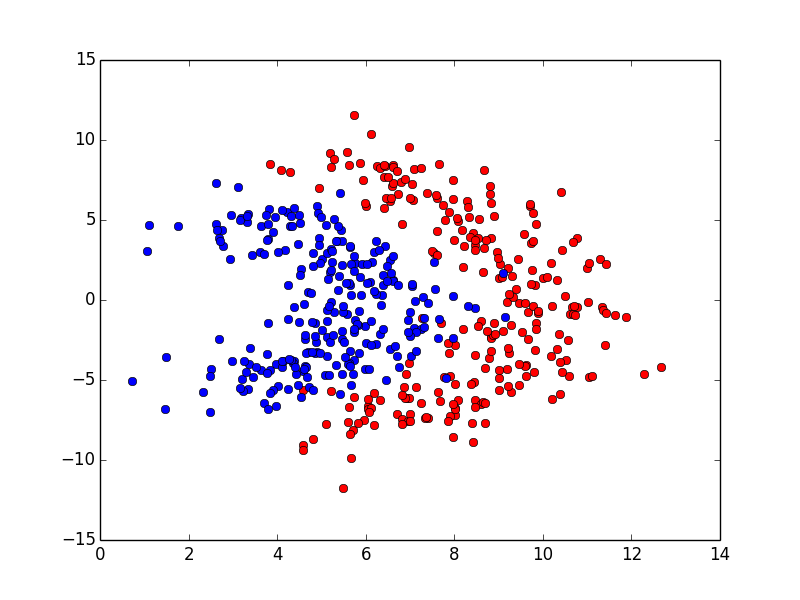
\includegraphics[scale=0.6]{figs/dataset_Lithuanian}
\caption{Lithuanian Data Set}
\label{Figure::lithuanian}
\end{figure}

\begin{figure}[]
\centering
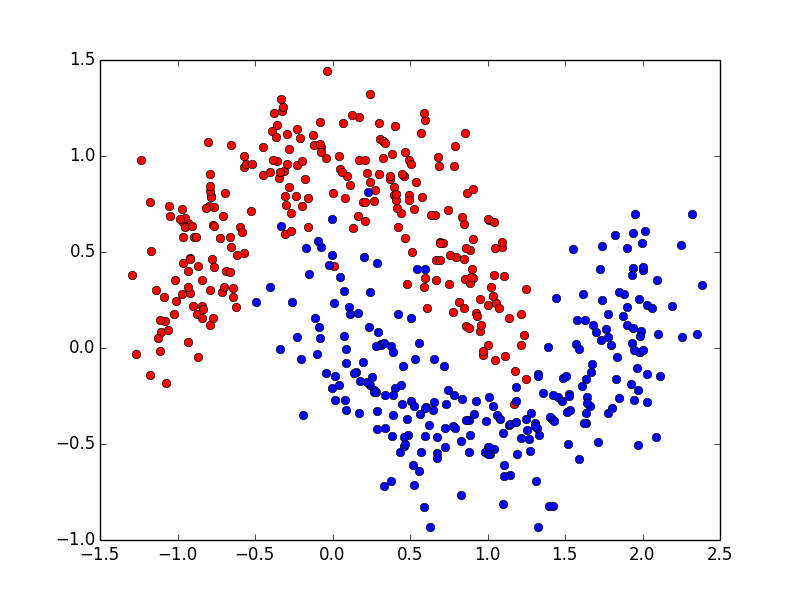
\includegraphics[scale=0.6]{figs/dataset_Banana}
\caption{Banana (Moon) Data Set}
\label{Figure::banana}
\end{figure}

\begin{figure}[]
\centering
\includegraphics[scale=0.6]{figs/dataset_Circle}
\caption{Circle Data Set}
\label{Figure::circle}
\end{figure}

Another purpose of this example is to show that we can reach the same level of detection by combining very simple and naive model detectors, instead of spending time to find the proper model and to train that model on the data set, which is usually a time consuming task. In this example, hundreds of linear detectors  are trained the data set. In order to have diverse learner detectors, we changed the ratio of data and their label during training to obtain as many diverse detectors as possible.

As shown below, we have different trained detectors on these data sets; none of them, however, can detect all the classes but as we will show later we can use them to better classify the data set by combining these simple detectors.

\begin{figure}[H]
\centering
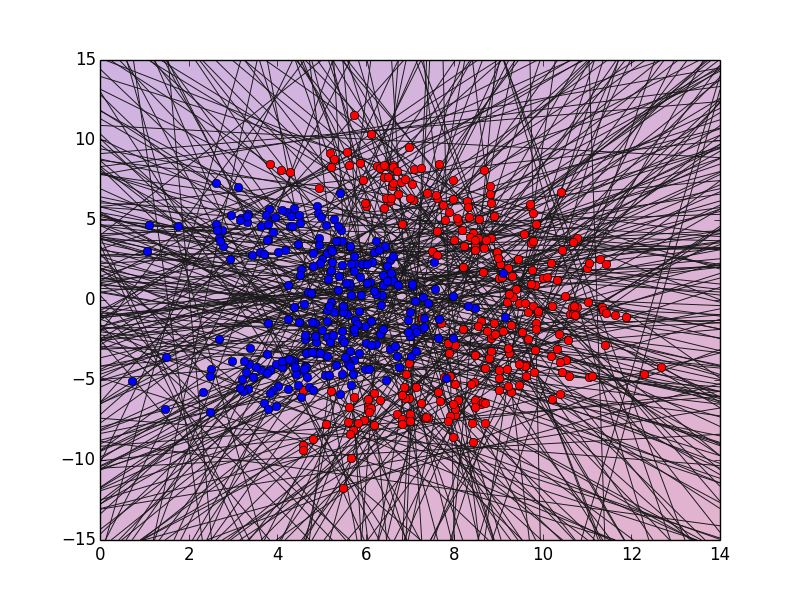
\includegraphics[scale=0.6]{figs/AllClassifiersLithuanian}
\caption{Linear detectors trained on the Lithuanian Data Set}
\label{Figure::lithuanian_all}
\end{figure}

\begin{figure}[H]
\centering
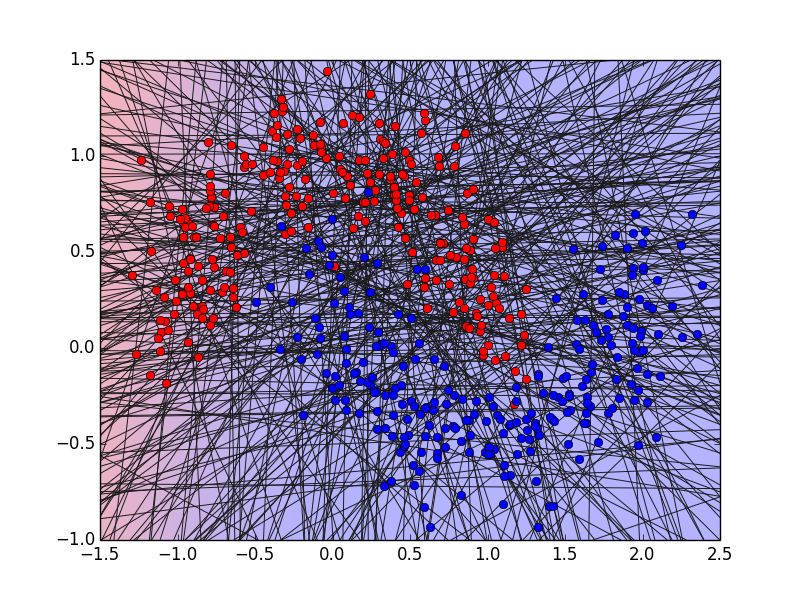
\includegraphics[scale=0.6]{figs/AllClassifiersBanana}
\caption{Linear detectors trained on the Banana (Moon) Data Set}
\label{Figure::banana_all}
\end{figure}

\begin{figure}[H]
\centering
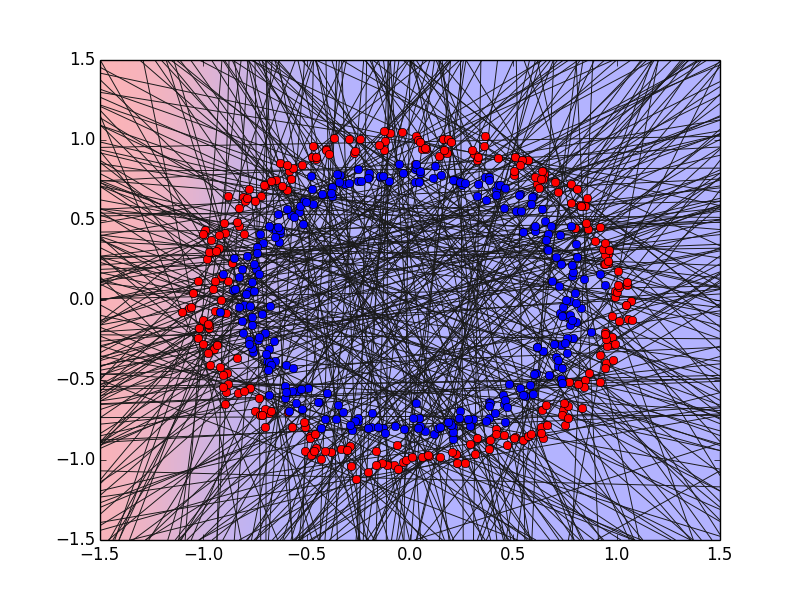
\includegraphics[scale=0.6]{figs/AllClassifiersCircle}
\caption{Linear detectors trained on the Circle Data Set}
\label{Figure::circle_all}
\end{figure}

By selecting the right models and combining them  we can increase the detection rate, as shown in Figures 2.7, 2.8 and 2.9. The figures on the left show the original detectors and their ROC before combination. After selecting the proper detectors and combining them together (after just one iteration) we can reach the accuracy shown on the right figures, which show the combined detectors (in yellow) and their improved ROC curve. The next step is to show why combination provides better results and how we can obtain the same result just by combining parts of trained models.



\begin{figure}[H]
    \centering
    \begin{adjustbox}{minipage=\linewidth,scale=1.1}
    \begin{subfigure}[b]{0.5\columnwidth}
        \centering
        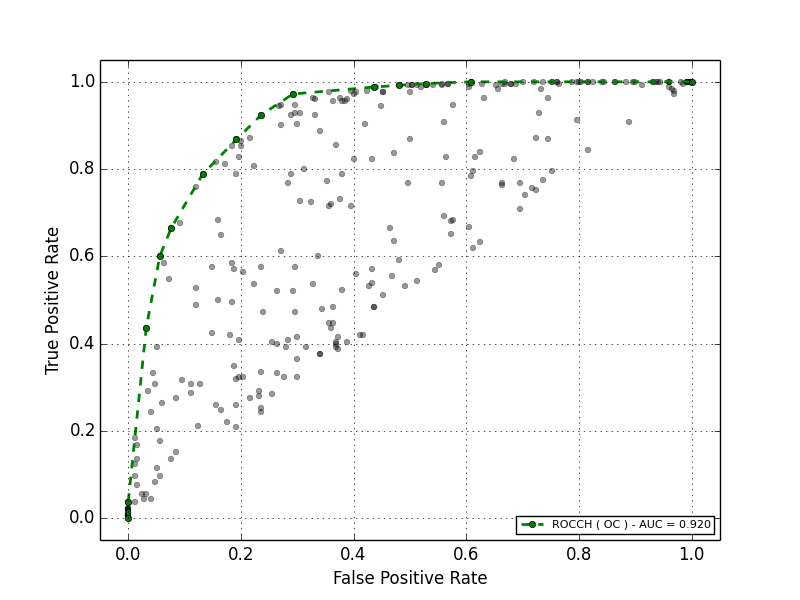
\includegraphics[width=\linewidth]{figs/ROCHLeft-Lithuanian}
        \caption{ROC before combination}
        \label{fig:ROC_left_lithuanian} 
    \end{subfigure}
    \begin{subfigure}[b]{0.5\columnwidth}
        \centering
        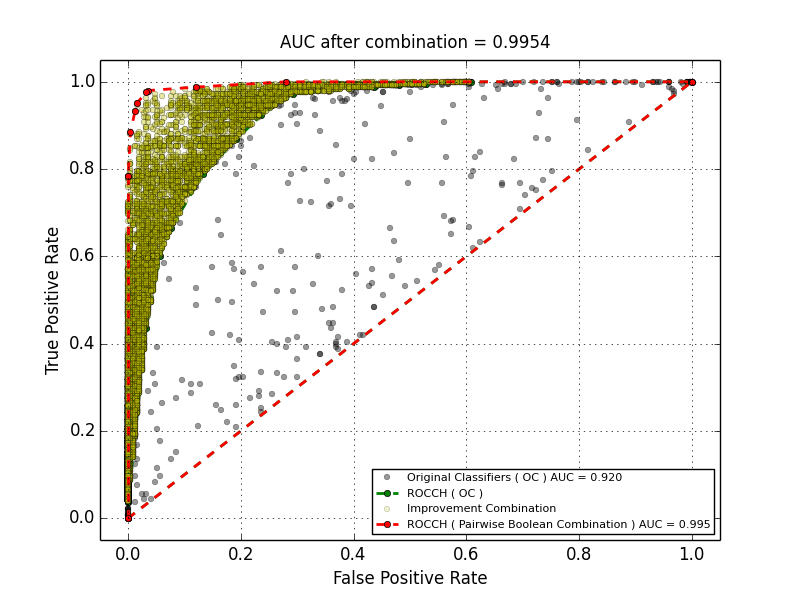
\includegraphics[width=\linewidth]{figs/ROCHRight-Lithuanian}
        \caption{ROC after combination}
        \label{fig:ROC_right_lithuanian}
    \end{subfigure}
    \caption{ROC comparison on Lithuanian data set before and after first round of combination}
    \label{fig:ROC_comparison_lithuanian}
    \end{adjustbox}
\end{figure}


\begin{figure}[H]
    \centering
    \begin{adjustbox}{minipage=\linewidth,scale=1.1}
    \begin{subfigure}[b]{0.5\columnwidth}
        \centering
        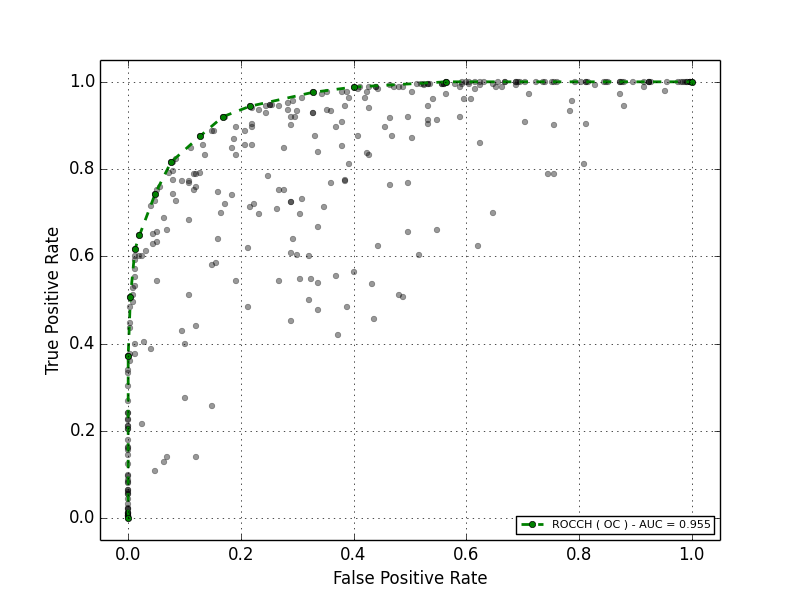
\includegraphics[width=\linewidth]{figs/ROCHLeft-Banana}
        \caption{ROC before combination}
        \label{fig:ROC_left_banana} 
    \end{subfigure}
    \begin{subfigure}[b]{0.5\columnwidth}
        \centering
        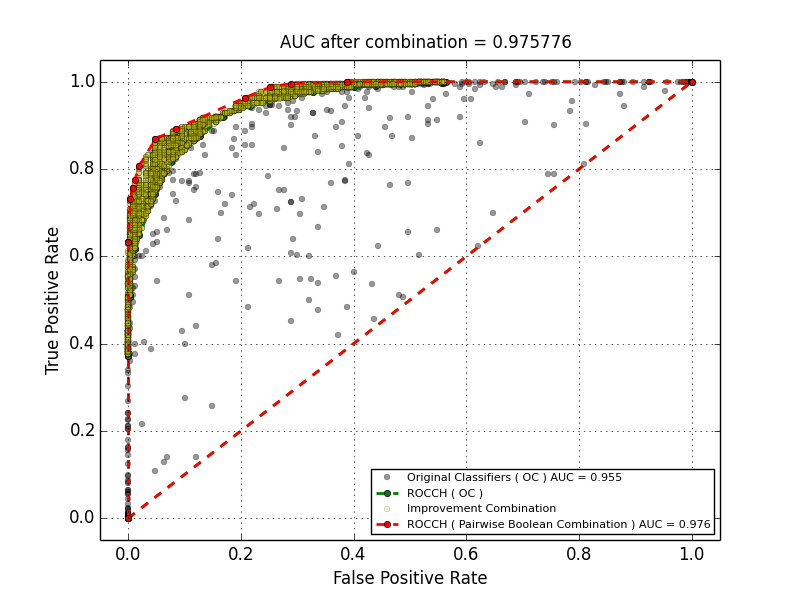
\includegraphics[width=\linewidth]{figs/ROCHRight-Banana}
        \caption{ROC after combination}
        \label{fig:ROC_right_banana}
    \end{subfigure}
    \caption{ROC comparison on Banana data set before and after first round of combination}
    \label{fig:ROC_comparison_banana}
    \end{adjustbox}
\end{figure}

\begin{figure}[H]
    \centering
    \begin{adjustbox}{minipage=\linewidth,scale=1.1}
    \begin{subfigure}[b]{0.5\columnwidth}
        \centering
        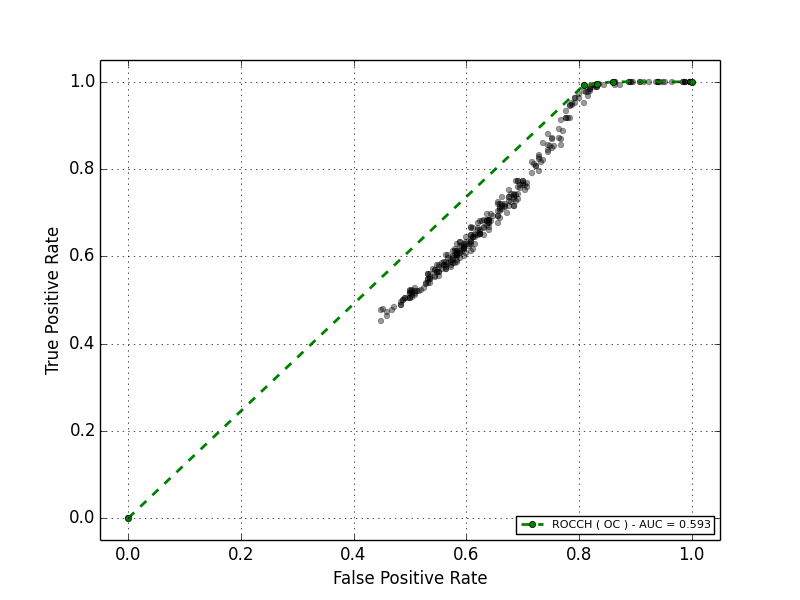
\includegraphics[width=\linewidth]{figs/ROCHLeft-Circle}
        \caption{ROC before combination}
        \label{fig:ROC_left_circle} 
    \end{subfigure}
    \begin{subfigure}[b]{0.5\columnwidth}
        \centering
        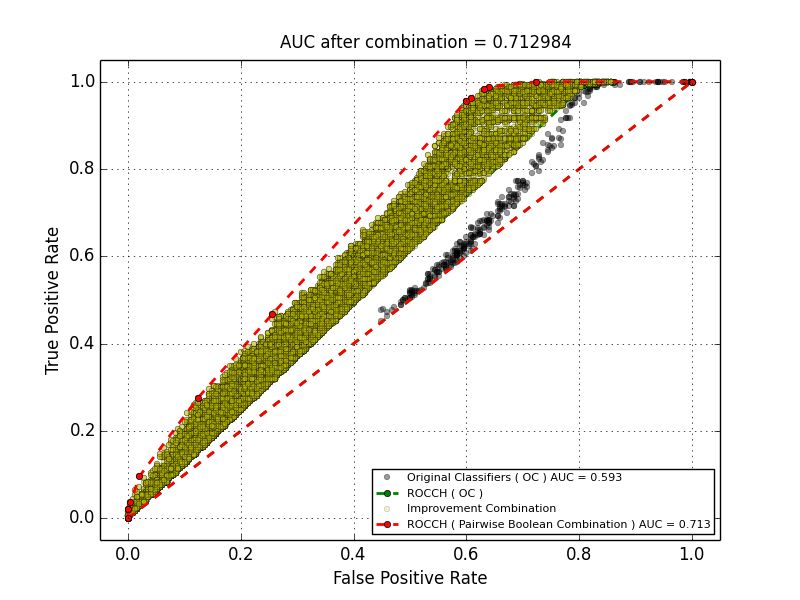
\includegraphics[width=\linewidth]{figs/ROCHRight-Circle}
        \caption{ROC after combination}
        \label{fig:ROC_right_circle}
    \end{subfigure}
    \caption{ROC comparison on Circle data set before and after first round of combination}
    \label{fig:ROC_comparison_circle}
    \end{adjustbox}
\end{figure}

For each data set, we show that there is no single detector that can classify the data set properly. 

\begin{figure}[t!] % "[t!]" placement specifier just for this example
\begin{subfigure}{0.48\textwidth}
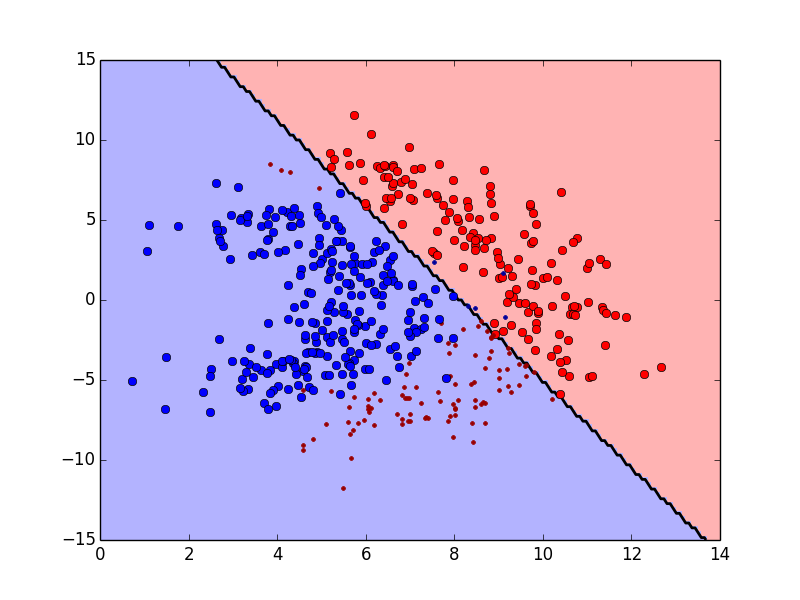
\includegraphics[width=\linewidth]{figs/Lithuanian/20All-Classifiers}
\caption{First subfigure} \label{fig:Lithuanian_all_single_a}
\end{subfigure}\hspace*{\fill}
\begin{subfigure}{0.48\textwidth}
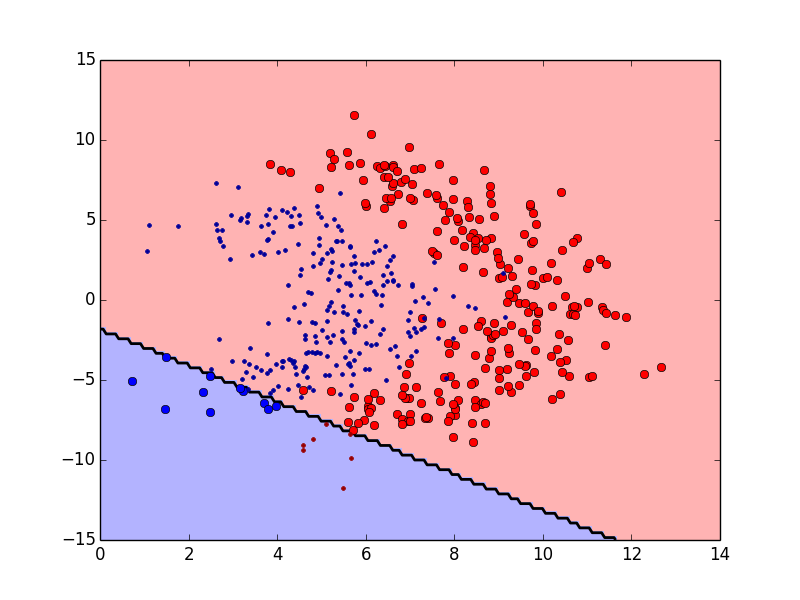
\includegraphics[width=\linewidth]{figs/Lithuanian/43All-Classifiers}
\caption{Second subfigure} \label{fig:Lithuanian_all_single_b}
\end{subfigure}

\medskip
\begin{subfigure}{0.48\textwidth}
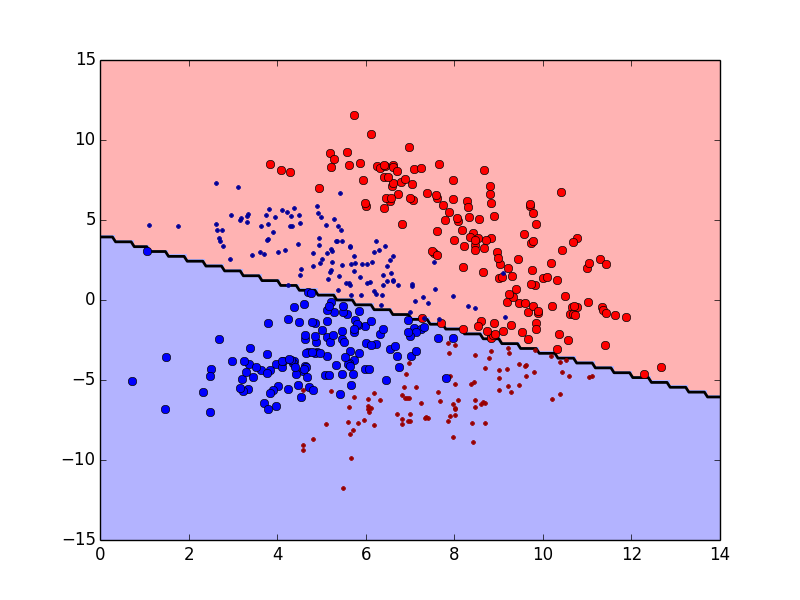
\includegraphics[width=\linewidth]{figs/Lithuanian/44All-Classifiers}
\caption{Third subfigure} \label{fig:Lithuanian_all_single_c}
\end{subfigure}\hspace*{\fill}
\begin{subfigure}{0.48\textwidth}
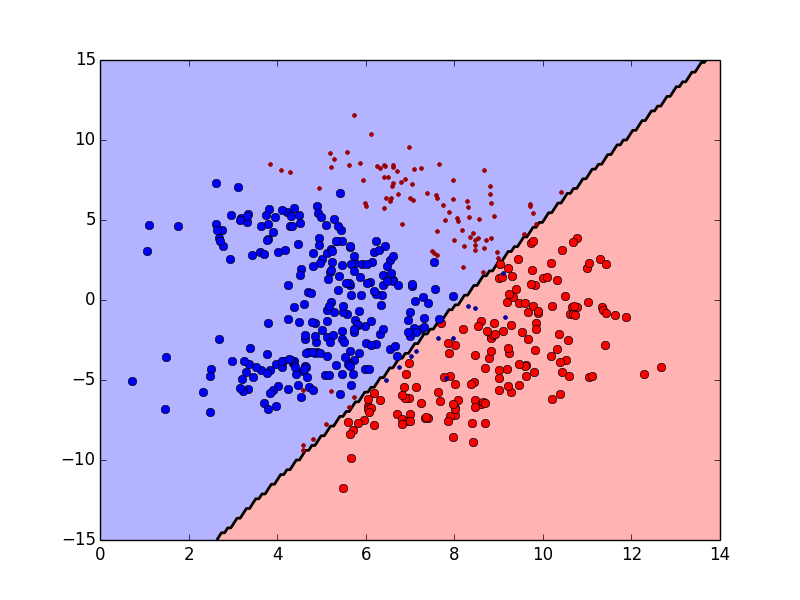
\includegraphics[width=\linewidth]{figs/Lithuanian/65All-Classifiers}
\caption{Fourth subfigure} \label{fig:Lithuanian_all_single_d}
\end{subfigure}

\medskip
\begin{subfigure}{0.48\textwidth}
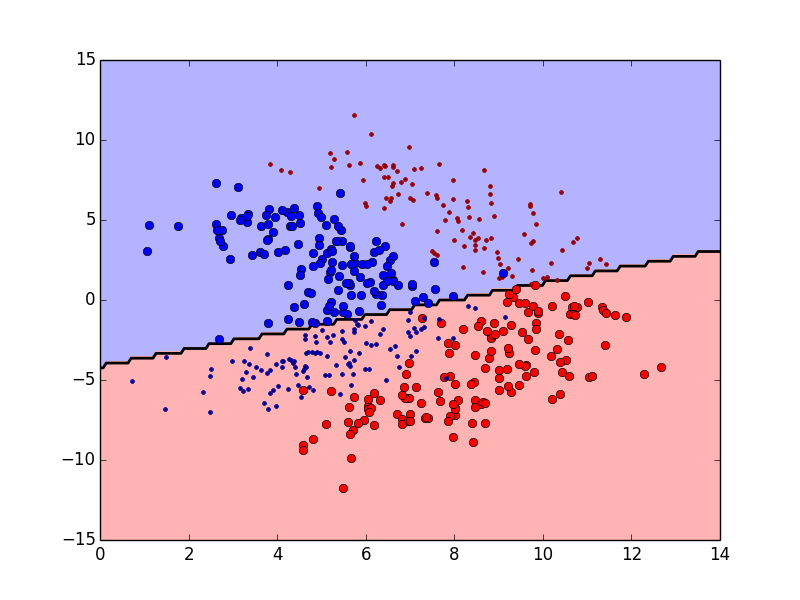
\includegraphics[width=\linewidth]{figs/Lithuanian/118All-Classifiers}
\caption{Fifth subfigure} \label{fig:Lithuanian_all_single_e}
\end{subfigure}\hspace*{\fill}
\begin{subfigure}{0.48\textwidth}
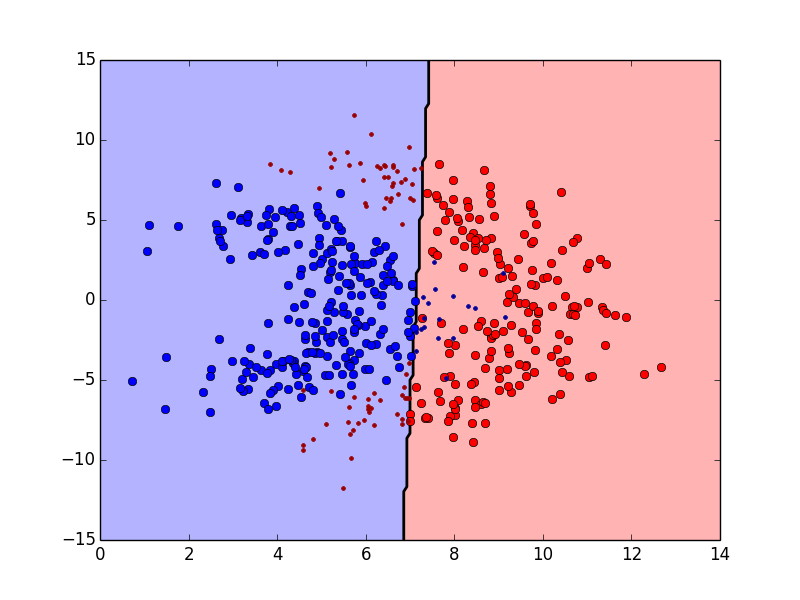
\includegraphics[width=\linewidth]{figs/Lithuanian/146All-Classifiers}
\caption{Sixth subfigure} \label{fig:Lithuanian_all_single_f}
\end{subfigure}

\caption{Some of best LDA ( Linear Discriminant Analysis) that can be trained on Lithuanian data set} \label{fig:Lithuanian_all_single}
\end{figure}

As it is shown in Figure~\ref{fig:Lithuanian_all_single}, with just one LDA, we cannot classify all the classes 100\%. We can, however, see that it is possible to choose two of these detectors and combine them to obtain a better result. As it is shown in Figure~\ref{fig:Dataset_ROC_Lithuanian}, we select detector from Figure~\ref{fig:Lithuanian_all_single_a}  and detectors from ~\ref{fig:Lithuanian_all_single_d} and combine them together.

\begin{figure}[H]
    \centering
    \begin{adjustbox}{minipage=\linewidth,scale=1.1}
    \begin{subfigure}[b]{0.5\columnwidth}
        \centering
        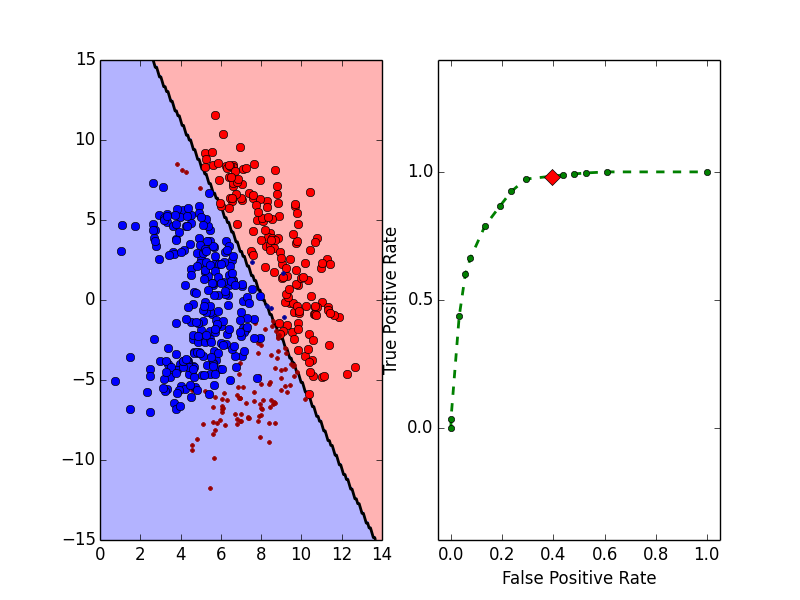
\includegraphics[width=\linewidth]{figs/Lithuanian/20Dataset-ROC}
        \caption{First selected LDA}
        \label{fig:Dataset_ROC_Lithuanian_a} 
    \end{subfigure}
    \begin{subfigure}[b]{0.5\columnwidth}
        \centering
        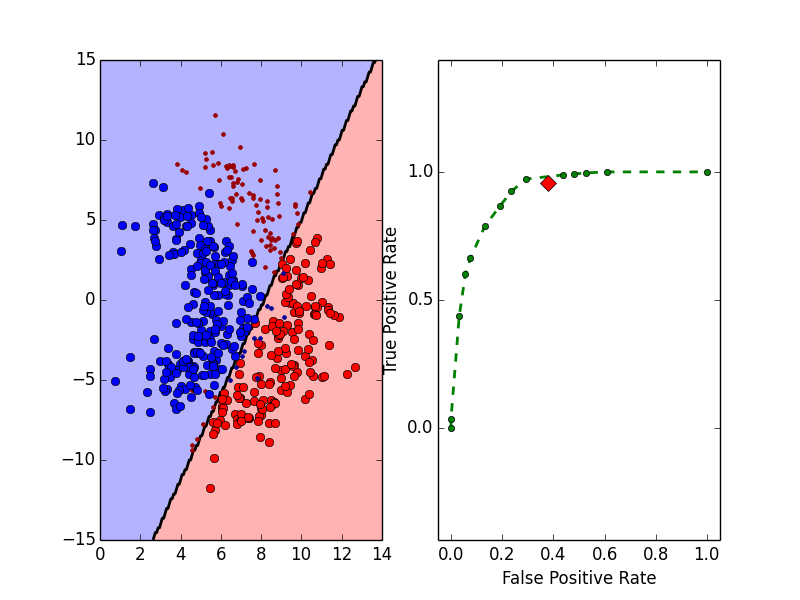
\includegraphics[width=\linewidth]{figs/Lithuanian/65Dataset-ROC}
        \caption{Second selected LDA}
        \label{fig:Dataset_ROC_Lithuanian_b}
    \end{subfigure}
    \caption{Selected LDA and their respective point compare to current ROC}
    \label{fig:Dataset_ROC_Lithuanian}
    \end{adjustbox}
\end{figure}

If we combine these two detectors with an $AND$ operation,  as shown in Figure~\ref{fig::combined_lithuanian_roc},  we can obtain a better result. The  red point is the mapping of the combined detectors. As we can see if we recalculate the ROC based on this new generated point we will have a greater AUC.

\begin{figure}[H]
\centering
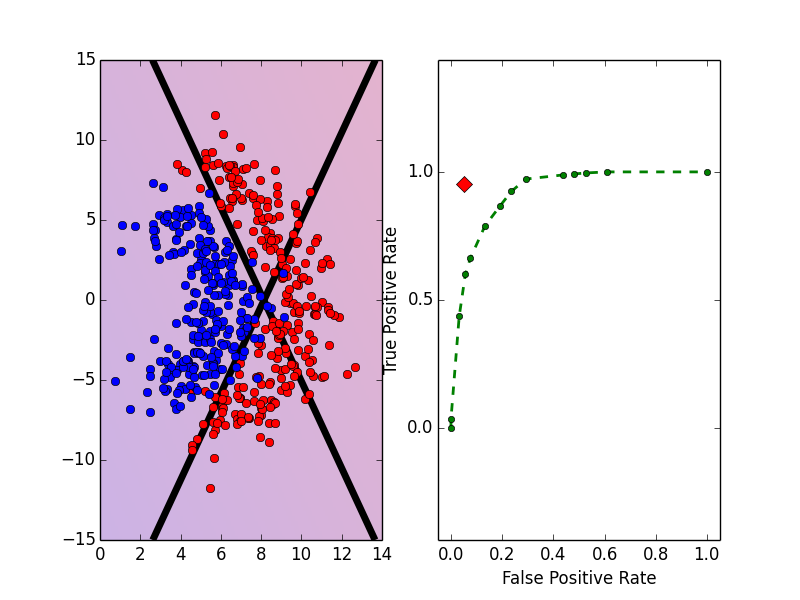
\includegraphics[scale=0.6]{figs/Lithuanian/9999999-combined_All-Classifiers}
\caption{Selected detectors and respective combined point on ROC curve}
\label{fig::combined_lithuanian_roc}
\end{figure}


A similar approach can be applied to the Banana data set. As you can see in Figure~\ref{fig:Banana_all_single}, like for the Lithuania data set, it is not possible to classify the data set completely with one detector.  In this specific example, we need at least three detectors in order to classify the data in an accurate way. 

\begin{figure}[t!] % "[t!]" placement specifier just for this example
\begin{subfigure}{0.48\textwidth}
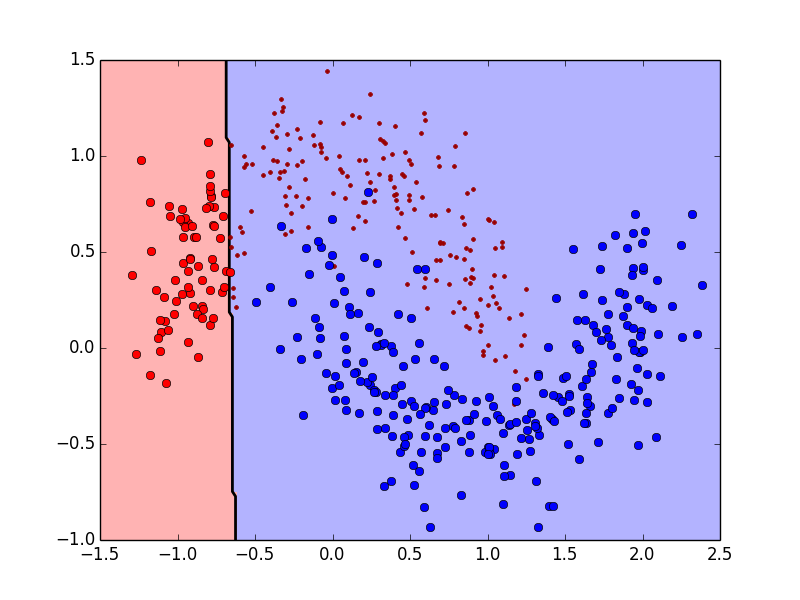
\includegraphics[width=\linewidth]{figs/Banana/2All-Classifiers}
\caption{First subfigure} \label{fig:Banana_all_single_a}
\end{subfigure}\hspace*{\fill}
\begin{subfigure}{0.48\textwidth}
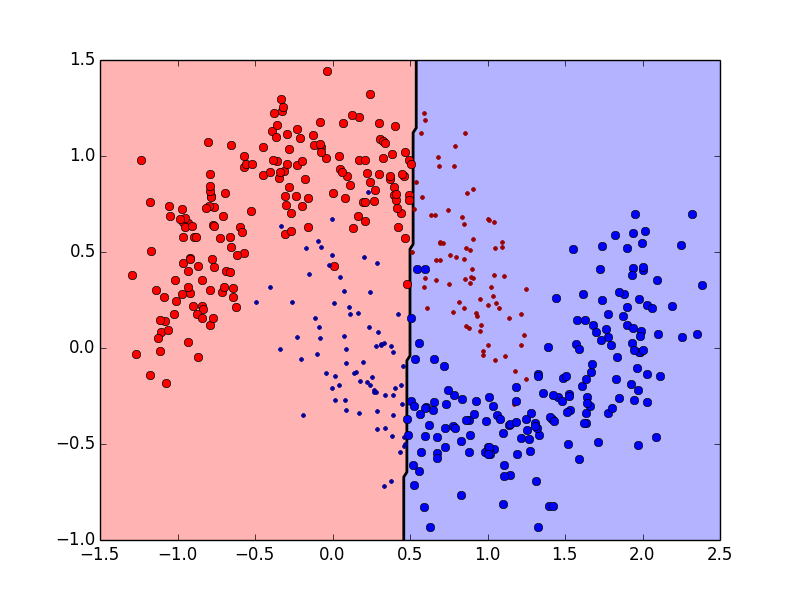
\includegraphics[width=\linewidth]{figs/Banana/12All-Classifiers}
\caption{Second subfigure} \label{fig:Banana_all_single_b}
\end{subfigure}

\medskip
\begin{subfigure}{0.48\textwidth}
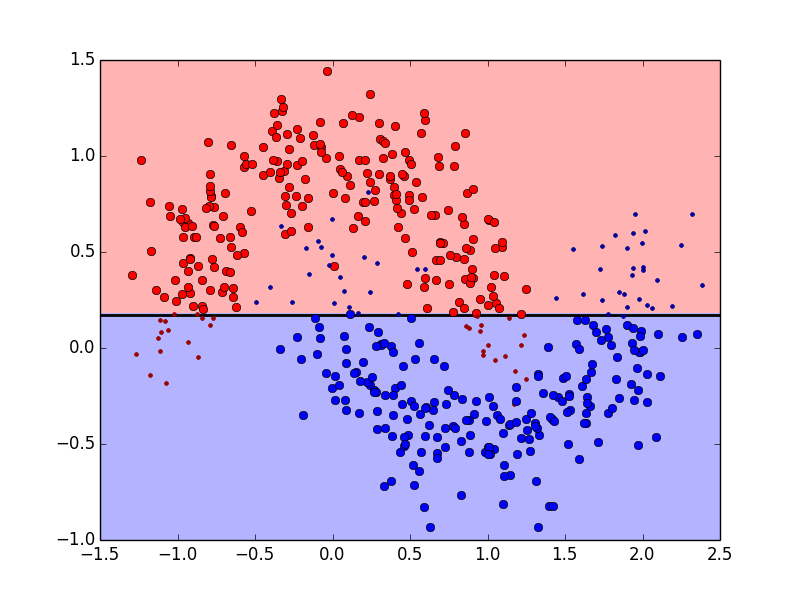
\includegraphics[width=\linewidth]{figs/Banana/22All-Classifiers}
\caption{Third subfigure} \label{fig:Banana_all_single_c}
\end{subfigure}\hspace*{\fill}
\begin{subfigure}{0.48\textwidth}
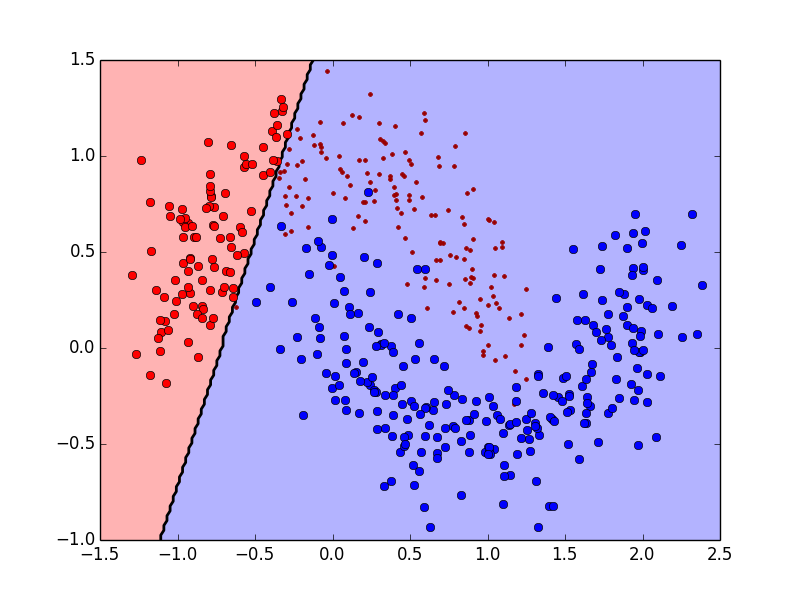
\includegraphics[width=\linewidth]{figs/Banana/54All-Classifiers}
\caption{Fourth subfigure} \label{fig:Banana_all_single_d}
\end{subfigure}

\medskip
\begin{subfigure}{0.48\textwidth}
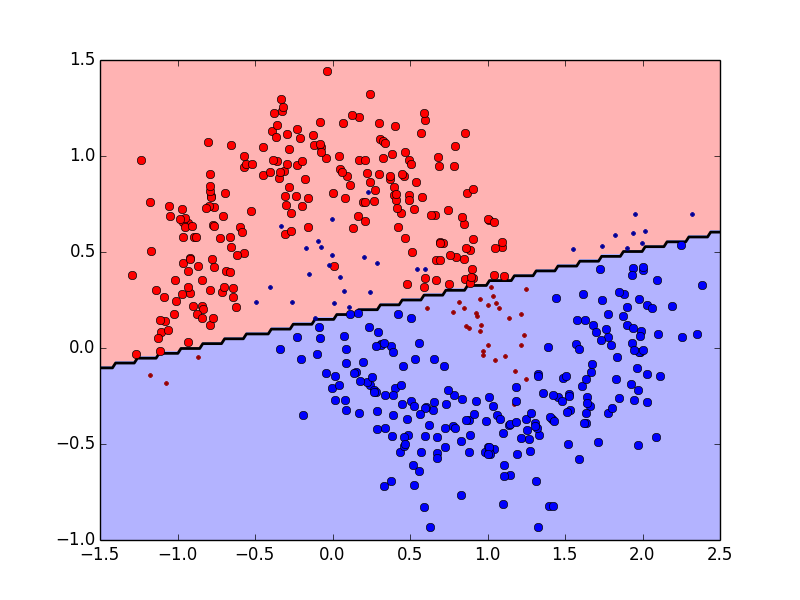
\includegraphics[width=\linewidth]{figs/Banana/147All-Classifiers}
\caption{Fifth subfigure} \label{fig:Banana_all_single_e}
\end{subfigure}\hspace*{\fill}
\begin{subfigure}{0.48\textwidth}
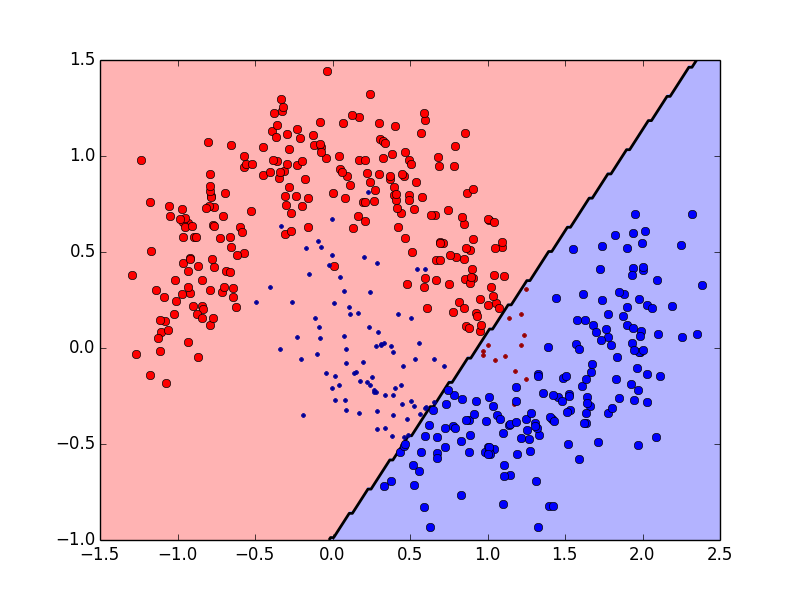
\includegraphics[width=\linewidth]{figs/Banana/160All-Classifiers}
\caption{Sixth subfigure} \label{fig:Banana_all_single_f}
\end{subfigure}

\caption{Some of best LDA ( Linear Discriminant Analysis) that can be trained on Banana data set} \label{fig:Banana_all_single}
\end{figure}

Based on the observation in this example it is better to select 3 detectors in order to be classify the data set, if we select detector in Figure~\ref{fig:Banana_all_single_a}, Figure~\ref{fig:Banana_all_single_c} and Figure~\ref{fig:Banana_all_single_f}  and combine them together we should expect to get the most accurate result among all other detectors. in figure~\ref{fig::combined_banana_roc} you can see all these detectors in one plot.


\begin{figure}[H]
\centering
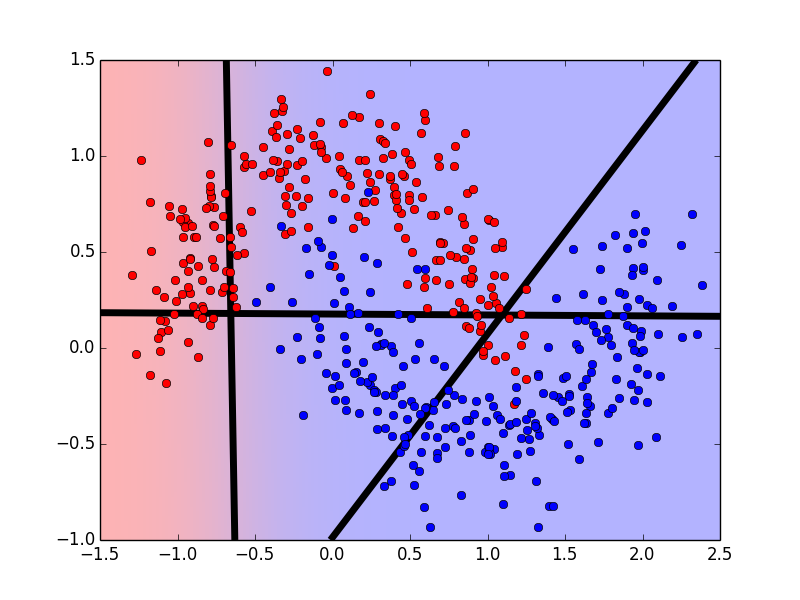
\includegraphics[scale=0.6]{figs/Banana/9999999-combined_selected_before_combination}
\caption{Best potential selected detectors on Banana data set}
\label{fig::combined_banana_roc}
\end{figure}

These examples show that it is not always necessary to train complex models, which takes time and resources, over the data set to obtain the best result possible. The same result can be achieved by combining two or more simple models, which can be trained much faster. Also by increasing the number these simple models, we can cover most of the cases (including the outliers) in the data set. Besides, even if we decide to train complex models, there is no guarantee that we can obtain the best results since every model has its own weaknesses. This said, some sort of combination is needed to help improve the result. In the next chapter we show how we can select a set of meaningful models that can help improve the result since it is not possible to train thousands of models and combine them all together. 

The Circle data set is a good example where doing combination in an iterative way improves the accuracy, as shown in Figure~\ref{fig:Circle_all_single}. We could not find any two detectors that can be combined  to classify the whole data set. What we need here is to select all of these detectors and start  combining them two by two iteratively. In Figure~\ref{fig::combined_circle_roc}, we show the result of classifying iteratively  the whole data set with the help of a few simple detectors.


\begin{figure}[H] % "[t!]" placement specifier just for this example
\begin{subfigure}{0.48\textwidth}
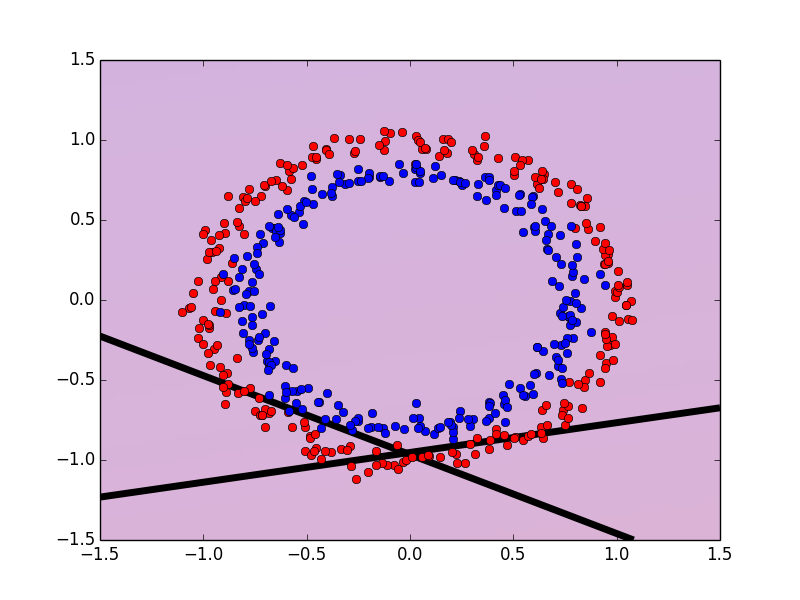
\includegraphics[width=\linewidth]{figs/Circle/11-two-circle}
\caption{First subfigure} \label{fig:Circle_all_single_a}
\end{subfigure}\hspace*{\fill}
\begin{subfigure}{0.48\textwidth}
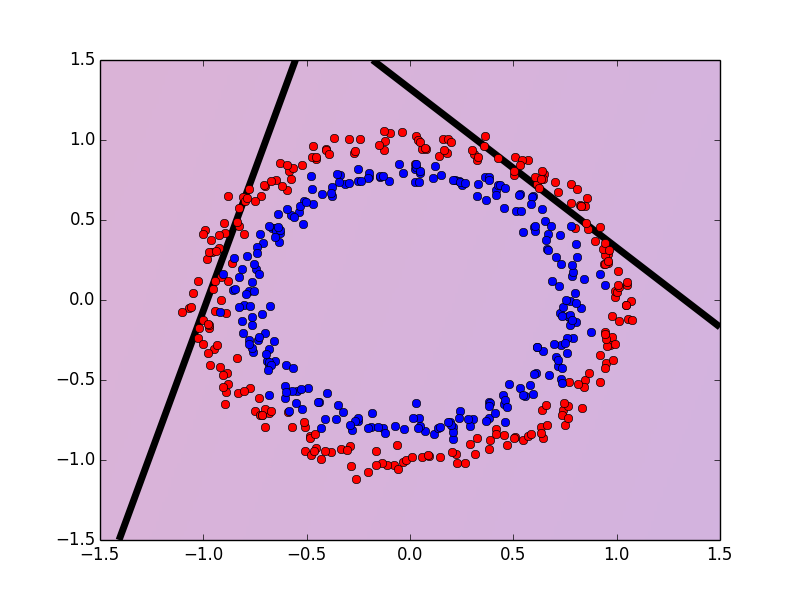
\includegraphics[width=\linewidth]{figs/Circle/22-two-circle}
\caption{Second subfigure} \label{fig:Circle_all_single_b}
\end{subfigure}

\medskip
\begin{subfigure}{0.48\textwidth}
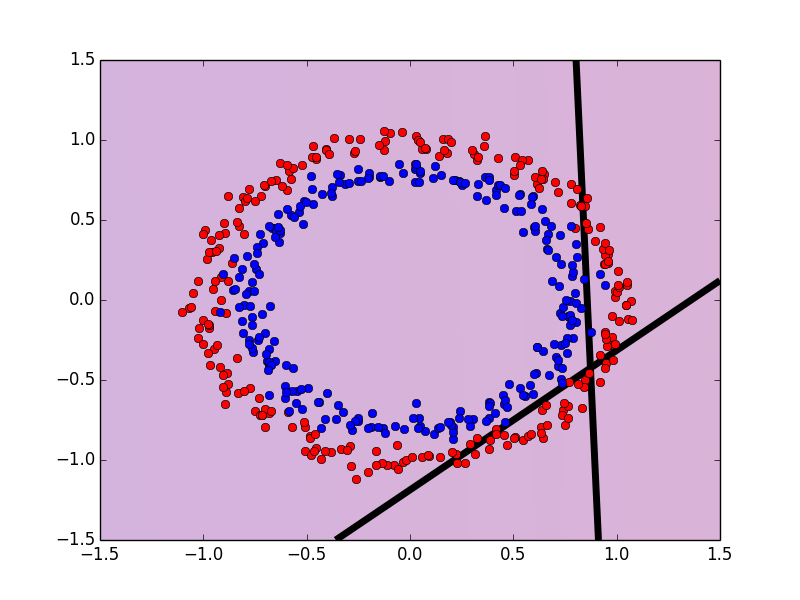
\includegraphics[width=\linewidth]{figs/Circle/33-two-circle}
\caption{Third subfigure} \label{fig:Circle_all_single_c}
\end{subfigure}\hspace*{\fill}
\begin{subfigure}{0.48\textwidth}
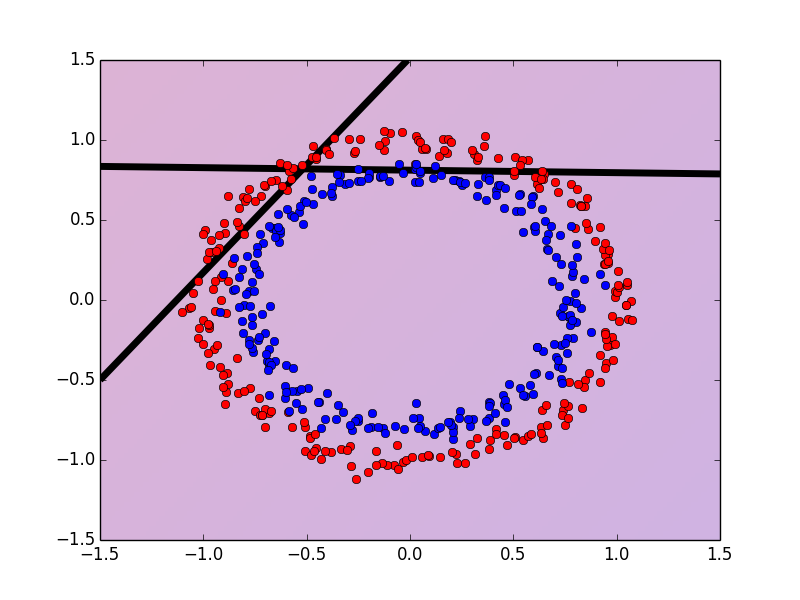
\includegraphics[width=\linewidth]{figs/Circle/44-two-circle}
\caption{Fourth subfigure} \label{fig:Circle_all_single_d}
\end{subfigure}

\medskip
\begin{subfigure}{0.48\textwidth}
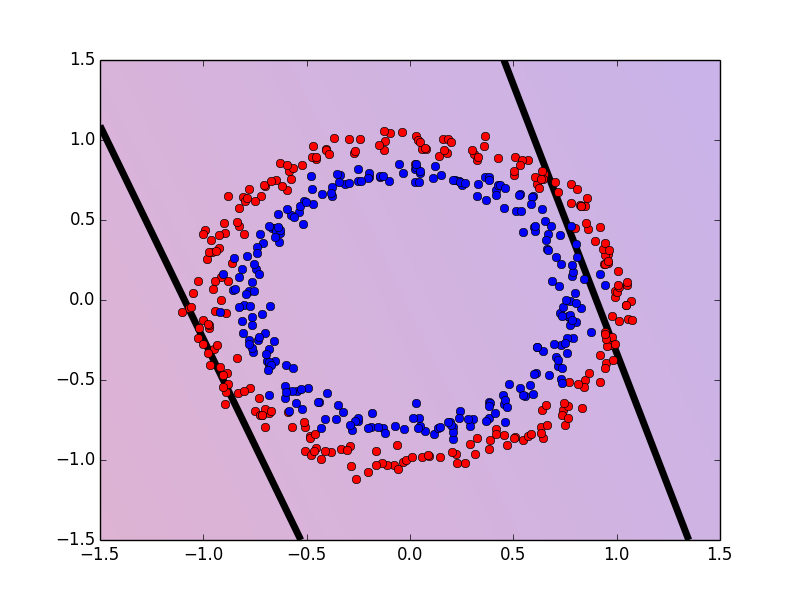
\includegraphics[width=\linewidth]{figs/Circle/55-two-circle}
\caption{Fifth subfigure} \label{fig:Circle_all_single_e}
\end{subfigure}\hspace*{\fill}
\begin{subfigure}{0.48\textwidth}
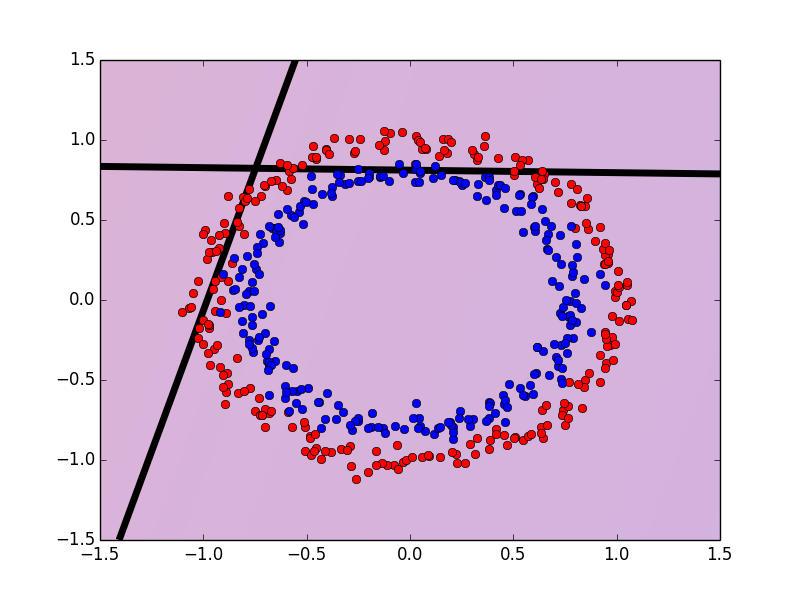
\includegraphics[width=\linewidth]{figs/Circle/66-two-circle}
\caption{Sixth subfigure} \label{fig:Circle_all_single_f}
\end{subfigure}

\caption{Series of 2 selected LDA ( Linear Discriminant Analysis) that can be trained and combined on the Circle data set} \label{fig:Circle_all_single}
\end{figure}

\begin{figure}[H]
\centering
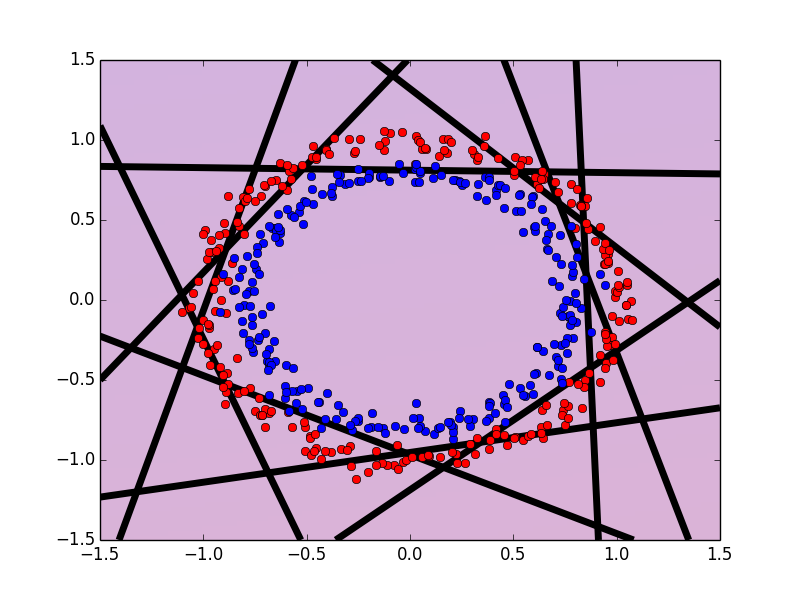
\includegraphics[scale=0.6]{figs/Circle/9999999-combined_selected_before_combination}
\caption{Best potential selected detectors on the Circle data set}
\label{fig::combined_circle_roc}
\end{figure}




